% arara: pdflatex
% !arara: indent: {overwrite: on}
\documentclass[aspectratio=169]{beamer}

\usepackage{ctex}

\usetheme{CambridgeUS}

\definecolor{frenchblue}{HTML}{0071BB}

%-change headline in each page-------------------------------
\setbeamercolor{palette tertiary}{fg=white, bg=frenchblue}
\setbeamertemplate{headline}
{
  \leavevmode%
  \hbox{%
  \begin{beamercolorbox}[wd=.6\paperwidth,ht=2.65ex,dp=1.5ex,center]{section in head/foot}%
    \usebeamerfont{section in head/foot}\thesection.\insertsectionhead\hspace*{2ex}
  \end{beamercolorbox}%
  \begin{beamercolorbox}[wd=.5\paperwidth,ht=2.65ex,dp=1.5ex,center]{subsection in head/foot}%
    \usebeamerfont{subsection in head/foot}\hspace*{2ex}\insertsubsectionhead
  \end{beamercolorbox}}%
  \vskip0pt%
}


%-change title part in each page-------------------------------
\setbeamercolor{frametitle}{fg=frenchblue,bg=white}


%-change foot part in each page-------------------------------
\makeatother
\setbeamertemplate{footline}
{
  \leavevmode%
  \hbox{%
  \begin{beamercolorbox}[wd=.0\paperwidth,ht=2.25ex,dp=1ex,center]{author in head/foot}%
    \usebeamerfont{author in head/foot}\insertshortauthor
  \end{beamercolorbox}%
  \begin{beamercolorbox}[wd=.63\paperwidth,ht=2.25ex,dp=1ex,center]{title in head/foot}%
    \usebeamerfont{title in head/foot}\textcolor{black}\insertshorttitle
  \end{beamercolorbox}%
  \begin{beamercolorbox}[wd=.37\paperwidth,ht=2.25ex,dp=1ex,center]{date in head/foot}% 
  \textcolor{black}\insertdate \hspace{0.2cm}
    \textcolor{black}\insertframenumber{} \textcolor{black}/ \textcolor{black}\inserttotalframenumber\hspace*{1ex}
  \end{beamercolorbox}}%
  \vskip0pt%
}
\makeatletter
\setbeamertemplate{navigation symbols}{}

%---remove headline for the Outline pages
\makeatletter
    \newenvironment{withoutheadline}{
        \setbeamertemplate{headline}[default]
        \def\beamer@entrycode{\vspace*{-\headheight}}
    }{}
\makeatother


%---remove headline and reset footline for publication list pages
\makeatletter
    \newenvironment{transparentFootline}{
	\setbeamertemplate{headline}[default]
        \def\beamer@entrycode{\vspace*{-\headheight}}
    
	\setbeamertemplate{footline}
		{
			\leavevmode%
			\hbox{%
		\pgfsetfillopacity{0}\begin{beamercolorbox}[wd=.63\paperwidth,ht=2.25ex,dp=1ex,center]{title in head/foot}%
			    \usebeamerfont{title in head/foot}\textcolor{black}\insertshorttitle
			  \end{beamercolorbox}%
		\pgfsetfillopacity{0}\begin{beamercolorbox}[wd=.37\paperwidth,ht=2.25ex,dp=1ex,center]{date in head/foot}% 
%\pgfsetfillopacity{1} \hspace{1.2cm}
\pgfsetfillopacity{1} \textcolor{black}\insertdate \hspace{0.2cm}
    \textcolor{black}\insertframenumber{} \textcolor{black}/ \textcolor{black}\inserttotalframenumber\hspace*{1ex}
  \end{beamercolorbox}
			}
			\vskip0pt%
		}
    }{}
\makeatother


%---remove headline and reset footline for last pages
\makeatletter
    \newenvironment{transparentFootline_lastpages}{
\setbeamertemplate{headline}
{
  \leavevmode%
  \hbox{%
  \pgfsetfillopacity{0}\begin{beamercolorbox}[wd=\paperwidth,ht=2.65ex,dp=1.5ex,center]{subsection in head/foot}empty\end{beamercolorbox}}%
  \pgfsetfillopacity{1}
  \vskip0pt%
}
        \setbeamertemplate{footline}
		{
			\leavevmode%
			\hbox{%
		\pgfsetfillopacity{0}\begin{beamercolorbox}[wd=.63\paperwidth,ht=2.25ex,dp=1ex,center]{title in head/foot}%
			    \usebeamerfont{title in head/foot}\textcolor{black}\insertshorttitle
			  \end{beamercolorbox}%
		\pgfsetfillopacity{0}\begin{beamercolorbox}[wd=.37\paperwidth,ht=2.25ex,dp=1ex,center]{date in head/foot}% 
%\pgfsetfillopacity{1} \hspace{1.2cm}
\pgfsetfillopacity{1} \textcolor{white}\insertdate \hspace{0.2cm}
    \textcolor{white}\insertframenumber{} \textcolor{white}/ \textcolor{white}\inserttotalframenumber\hspace*{1ex}
  \end{beamercolorbox}
			}
			\vskip0pt%
		}
    }{}
\makeatother


%---change color of items in enumerate environment--
\setbeamertemplate{enumerate items}[default]

\usepackage{bm}
\usepackage{comment}
\usepackage{graphics} % used for scalebox
\usepackage{multirow}%used for multicolumn
\usepackage{array}%used for vrule
\usepackage{subfigure}
\usepackage{threeparttable} % used for footnotes in table

%---set tikz highlighter------------------------
\usepackage{multirow, booktabs, dcolumn, color} % Tables
\usepackage[beamer,customcolors]{hf-tikz}
\usetikzlibrary{calc}
% To set the hypothesis highlighting boxes red.
\tikzset{hl/.style={
    set fill color=red!80!black!40,
    set border color=red!80!black,
  },
}
%-----------------------------------------------

%---set tikz marker-----------------------------
\usepackage{tikz}
\usetikzlibrary{positioning}
\tikzset{>=stealth}

\newcommand{\tikzmark}[3][]{\tikz[overlay,remember picture,baseline] \node [anchor=base,#1](#2) {#3};}
%-----------------------------------------------

%---set textblock----------------------------
\usepackage[absolute,overlay]{textpos}
%--------------------------------------------------------

%use bold arrow
\usepackage{marvosym}

%used for aligning the figure to left
\usepackage[export]{adjustbox}

%used for colored block
\usepackage[listings,theorems]{tcolorbox}

%used for algorithm
\usepackage[ruled,vlined,linesnumbered]{algorithm2e}
\usepackage{algorithmic}


%########################################
%########################################
% Custom title page
\setbeamertemplate{title page}
{
  %\vskip-0.59cm%
  \hskip13.0cm%
  \inserttitlegraphic%
  \vfill%
    \begin{beamercolorbox}[sep=12pt]{title}
      \ifx\insertsubtitle\@empty%
      \else%
        {\usebeamerfont{subtitle}\usebeamercolor[fg]{subtitle}\begin{tikzpicture}
			\node[fill=frenchblue,draw=frenchblue, text=white] at (0,0) {\insertsubtitle};
			\end{tikzpicture}
		}%
        \vskip0.25em%
      \fi%
      %\begin{center} \line(1,0){450} \end{center}
	  \usebeamerfont{title}\textcolor{frenchblue}\inserttitle\par%
    \end{beamercolorbox}%
    
    \vskip2em\par
    
    \begin{beamercolorbox}[sep=6pt]{author}
      \hskip23.5em \usebeamerfont{author}\insertauthor
    \end{beamercolorbox}
    \begin{beamercolorbox}[sep=6pt]{institute}
      \hskip21em \usebeamerfont{institute}\insertinstitute
    \end{beamercolorbox}
    \begin{beamercolorbox}[sep=6pt]{date}
      \hskip25em \usebeamerfont{date}\insertdate
    \end{beamercolorbox}
  \vfill
}

\titlegraphic{
\includegraphics[width=1cm]{pkulogo}
}

\title{基于知识迁移的社交媒体事件检测方法研究}
\subtitle{博士论文答辩报告}
\author{博士生:黄威靖\\ \hskip23em 导师:王腾蛟教授}
\institute{北京大学信息科学技术学院数据库实验室}
\date{2018-06-05}
%########################################
%########################################

\begin{document}


\begin{frame}[plain]
\maketitle
\end{frame}


%TODO 制作导航部分
\begin{withoutheadline}
\begin{frame}
\vspace*{-13mm}
\begin{figure}
	\hspace*{-4.2mm}
    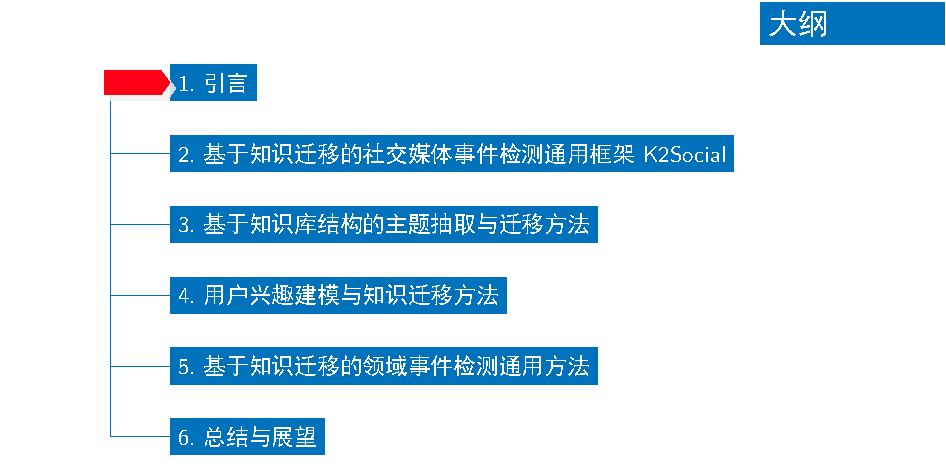
\includegraphics[width=1.0\paperwidth]{img/contents1_output.pdf}
\end{figure}
\end{frame}
\end{withoutheadline}

\section{引言}
%------------------------------
%page 2
\begin{frame}
\frametitle{Motivation}

Many Web applications need the \textbf{accurate event detection} technique on microblog stream, including:
\begin{enumerate}
	%\item 公共舆情分析 [Chen, SIGIR 2013]
	%\item {\kaishu \textbf{公共安全}} [Li, ICDE 2012], [Imran, WWW 2014]
	\item disaster response [Sakaki,WWW 2010]
	\item breaking news report\footnote{\url{http://www.theverge.com/2016/12/1/13804542/reuters-algorithm-breaking-news-twitter}}
\end{enumerate}	
\vfill

But detecting events on twitter stream accurately is still challenging.
\end{frame}


%TODO 制作导航部分
\begin{withoutheadline}
\begin{frame}
\vspace*{-13mm}
\begin{figure}
	\hspace*{-4.2mm}
    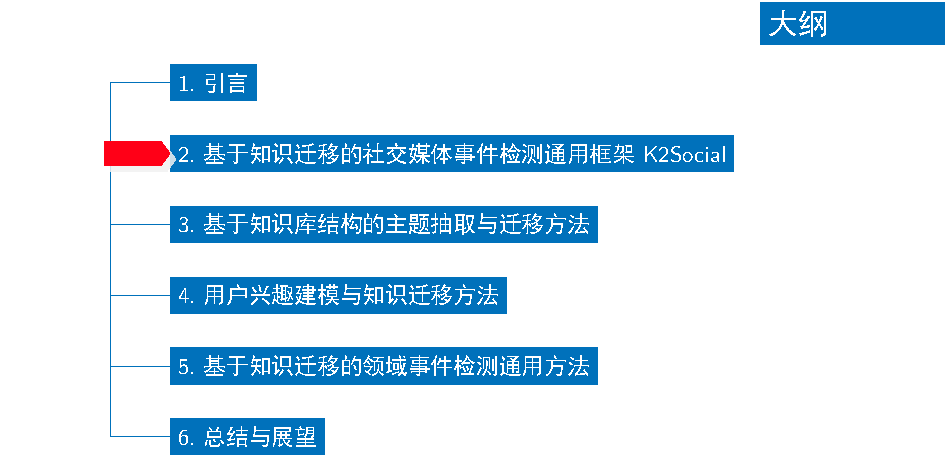
\includegraphics[width=1.0\paperwidth]{img/contents2_output.pdf}
\end{figure}

\end{frame}
\end{withoutheadline}

\section{基于知识迁移的社交媒体事件检测通用框架K2Social}
%------------------------------
%page 2
\begin{frame}
\frametitle{Motivation}

Many Web applications need the \textbf{accurate event detection} technique on microblog stream, including:
\begin{enumerate}
	%\item 公共舆情分析 [Chen, SIGIR 2013]
	%\item {\kaishu \textbf{公共安全}} [Li, ICDE 2012], [Imran, WWW 2014]
	\item disaster response [Sakaki,WWW 2010]
	\item breaking news report\footnote{\url{http://www.theverge.com/2016/12/1/13804542/reuters-algorithm-breaking-news-twitter}}
\end{enumerate}	
\vfill

But detecting events on twitter stream accurately is still challenging.
\end{frame}


%TODO 制作导航部分
\begin{frame}[plain]
\vspace*{-9.5mm}
\begin{figure}
	\hspace*{-4.2mm}
    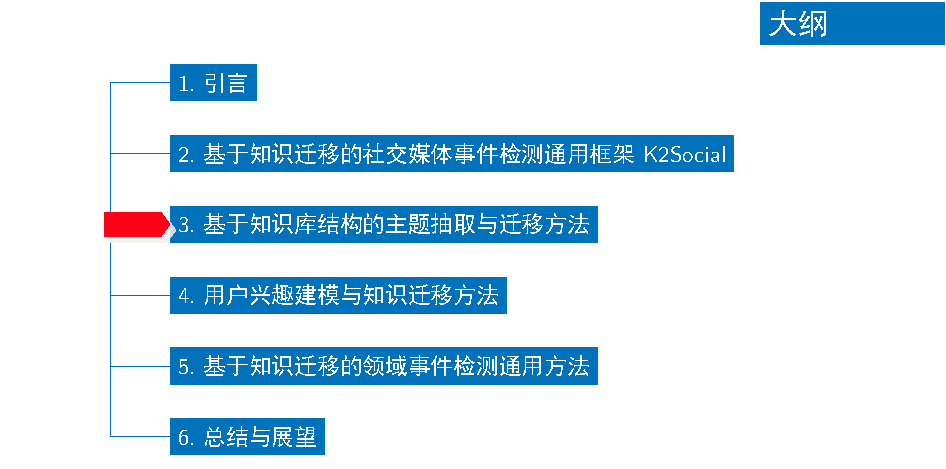
\includegraphics[width=1.0\paperwidth]{img/contents3_output.pdf}
\end{figure}

\end{frame}

\section{基于知识库结构的主题抽取与迁移方法}
%------------------------------
%page 2
\begin{frame}
\frametitle{Motivation}

Many Web applications need the \textbf{accurate event detection} technique on microblog stream, including:
\begin{enumerate}
	%\item 公共舆情分析 [Chen, SIGIR 2013]
	%\item {\kaishu \textbf{公共安全}} [Li, ICDE 2012], [Imran, WWW 2014]
	\item disaster response [Sakaki,WWW 2010]
	\item breaking news report\footnote{\url{http://www.theverge.com/2016/12/1/13804542/reuters-algorithm-breaking-news-twitter}}
\end{enumerate}	
\vfill

But detecting events on twitter stream accurately is still challenging.
\end{frame}


%TODO 制作导航部分
\begin{withoutheadline}
\begin{frame}
\vspace*{-13mm}
\begin{figure}
	\hspace*{-4.2mm}
    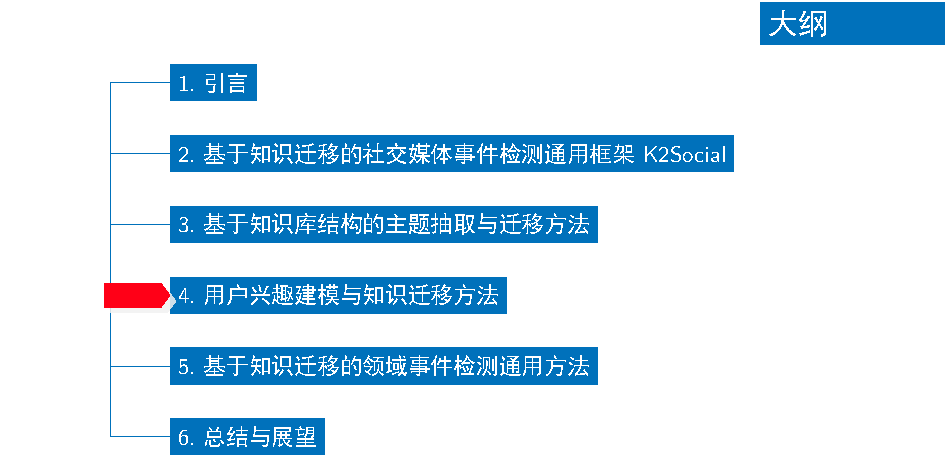
\includegraphics[width=1.0\paperwidth]{img/contents4_output.pdf}
\end{figure}

\end{frame}
\end{withoutheadline}

\section{用户兴趣建模与知识迁移方法}
%------------------------------
%page 2
\begin{frame}
\frametitle{Motivation}

Many Web applications need the \textbf{accurate event detection} technique on microblog stream, including:
\begin{enumerate}
	%\item 公共舆情分析 [Chen, SIGIR 2013]
	%\item {\kaishu \textbf{公共安全}} [Li, ICDE 2012], [Imran, WWW 2014]
	\item disaster response [Sakaki,WWW 2010]
	\item breaking news report\footnote{\url{http://www.theverge.com/2016/12/1/13804542/reuters-algorithm-breaking-news-twitter}}
\end{enumerate}	
\vfill

But detecting events on twitter stream accurately is still challenging.
\end{frame}


%TODO 制作导航部分
\begin{withoutheadline}
\begin{frame}
\vspace*{-13mm}
\begin{figure}
	\hspace*{-4.2mm}
    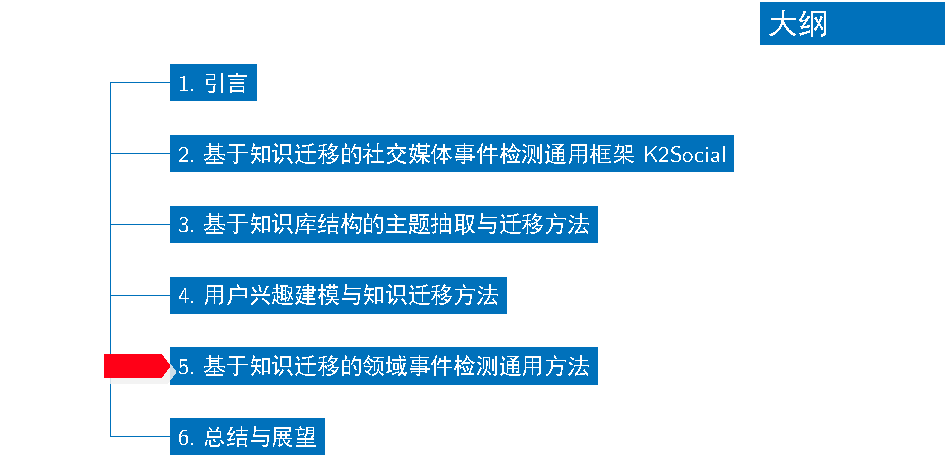
\includegraphics[width=1.0\paperwidth]{img/contents5_output.pdf}
\end{figure}

\end{frame}
\end{withoutheadline}

\section{基于知识迁移的领域事件检测通用方法}
%------------------------------
%page 2
\begin{frame}
\frametitle{Motivation}

Many Web applications need the \textbf{accurate event detection} technique on microblog stream, including:
\begin{enumerate}
	%\item 公共舆情分析 [Chen, SIGIR 2013]
	%\item {\kaishu \textbf{公共安全}} [Li, ICDE 2012], [Imran, WWW 2014]
	\item disaster response [Sakaki,WWW 2010]
	\item breaking news report\footnote{\url{http://www.theverge.com/2016/12/1/13804542/reuters-algorithm-breaking-news-twitter}}
\end{enumerate}	
\vfill

But detecting events on twitter stream accurately is still challenging.
\end{frame}


%TODO 制作导航部分
\begin{frame}[plain]
\vspace*{-9.5mm}
\begin{figure}
	\hspace*{-4.2mm}
    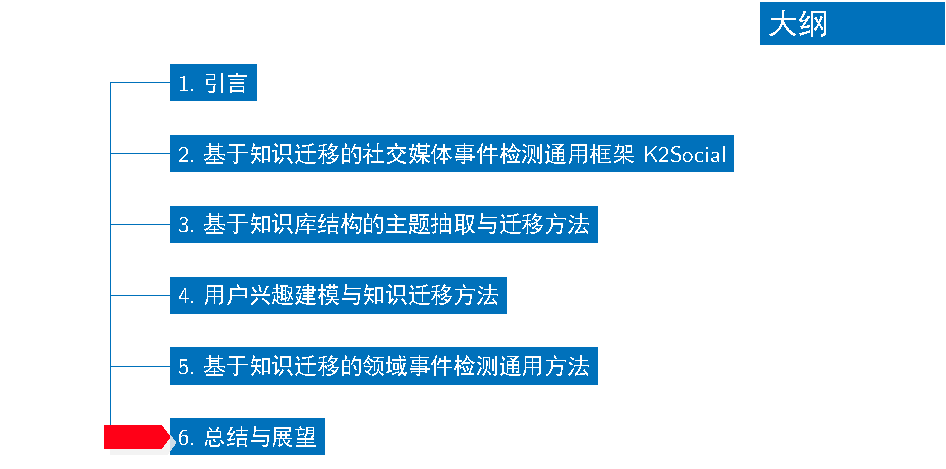
\includegraphics[width=1.0\paperwidth]{img/contents6_output.pdf}
\end{figure}

\end{frame}

\section{总结与展望}
%------------------------------
%page 2
\begin{frame}
\frametitle{Motivation}

Many Web applications need the \textbf{accurate event detection} technique on microblog stream, including:
\begin{enumerate}
	%\item 公共舆情分析 [Chen, SIGIR 2013]
	%\item {\kaishu \textbf{公共安全}} [Li, ICDE 2012], [Imran, WWW 2014]
	\item disaster response [Sakaki,WWW 2010]
	\item breaking news report\footnote{\url{http://www.theverge.com/2016/12/1/13804542/reuters-algorithm-breaking-news-twitter}}
\end{enumerate}	
\vfill

But detecting events on twitter stream accurately is still challenging.
\end{frame}


%------------------------------
%page 1
\begin{transparentFootline}
\begin{frame}
\frametitle{论文发表情况(1/3)}

\footnotesize
\begin{enumerate}
\item \textbf{Weijing Huang}, Tengjiao Wang, Wei Chen, Siyuan Jiang, Kam-Fai Wong, PhraseCTM: Correlated Topic Modeling on Phrases within Markov Random Fields, ACL 2018, accepted, to appear. (CCF A类) 
\item \textbf{Weijing Huang}, Tengjiao Wang, Wei Chen, Yazhou Wang, Category-Level Transfer Learning from Knowledge Base to Microblog Stream for Accurate Event Detection, DASFAA 2017. (EI index number: 20174404323179, CCF B类)
\item \textbf{Weijing Huang}, Wei Chen, Tengjiao Wang, Shibo Tao. TaxoPhrase: Exploring Knowledge Base via Joint Learning of Taxonomy and Topical Phrases, the 2nd Open Knowledge Base and Question Answering Workshop at SIGIR 2017.
\item \textbf{Weijing Huang}, Wei Chen, Tengjiao Wang, Shibo Tao. Efficient Topic Modeling on Phrases via Sparsity, the 29th IEEE International Conference on Tools with Artificial Intelligence (ICTAI) 2017, accepted, to appear. 
\item \textbf{Weijing Huang}, Wei Chen, Lamei Zhang, Tengjiao Wang, An Efficient Online Event Detection Method for Microblogs via User Modeling, the 18th Asia Pacific Web Conference (APWeb) 2016. (EI index number: 20164102880250)
\end{enumerate}
\end{frame}
\end{transparentFootline}

%------------------------------
%page 2
\begin{transparentFootline}
\begin{frame}
\frametitle{论文发表情况(2/3)}

\footnotesize
\begin{enumerate}\addtocounter{enumi}{5}
\item Ruhui Wang, \textbf{Weijing Huang}, Wei Chen, Tengjiao Wang, Kai Lei. ASEM: Mining Aspects and Sentiment of Events from Microblog, the 24th ACM International Conference on Information and Knowledge Management (CIKM) 2015.
\item Yue Wang, \textbf{Weijing Huang}, Lang Zong, Tengjiao Wang, Dongqing Yang: Influence maximization with limit cost in social network. SCIENCE CHINA Information Sciences 56(7): 1-14 (2013) 
\item Yue Wang, \textbf{Weijing Huang}, Wei Chen, Tengjiao Wang,Dongqing Yang. Informed Prediction with Incremental Core-based Friend Cycle Discovering, the 12th International Conference on Web-Age Information Management (WAIM) 2011. 
\item 张腊梅,\textbf{黄威靖},陈薇,王腾蛟,雷凯. EMTM:微博中与主题相关的专家挖掘方法. 计算机研究与发展. 2016年(第53卷)(萨师煊优秀学生论文奖).
\item 吴良, \textbf{黄威靖}, 陈薇, 王腾蛟, 雷凯, 刘月琴. ACT-LDA: 集成话题、社区和影响力分析的概率模型. 计算机科学与探索. 2013年第7卷第8期(718-728). 
\end{enumerate}
\end{frame}
\end{transparentFootline}

%------------------------------
%page 3
\begin{transparentFootline}
\begin{frame}
\frametitle{论文发表情况(3/3)}

\footnotesize
\begin{enumerate}\addtocounter{enumi}{10}
\item Shibo Tao, Xiaorong Wang, \textbf{Weijing Huang}, Wei Chen, Tengjiao Wang, Kai Lei, From Citation Network to Study Map: A Novel Model to Reorganize Academic Literatures, Big Scholar workshop at WWW 2017.
\item Wei Chen, Lang Zong, \textbf{Weijing Huang}, Gaoyan Ou, Yue Wang, Dongqing Yang, An Empirical Study of Massively Parallel Bayesian Networks Learning for Sentiment Extraction from Unstructured Text, the 13th Asia-Pacific Web Conference (APWeb) 2011. 
\item Xilian Li, Wei Chen, Tengjiao Wang, \textbf{Weijing Huang}, Target-specific Convolutional Bi-directional LSTM Neural Network for Political Ideology Analysis, the Asia Pacific Web and Web-Age Information Management Joint Conference on Web and Big Data (APWeb-WAIM) 2017.
\item Xiao Zhang, Xiaorong Wang, Wei Chen, Jie Tao, \textbf{Weijing Huang}, Tengjiao Wang, A Taxi Gap Prediction Method via Double Ensemble Gradient Boosting Decision Tree, the 2nd IEEE International Conference on Intelligent Data and Security 2017.
\end{enumerate}
\end{frame}
\end{transparentFootline}

%------------------------------
%page 4
\begin{transparentFootline}
\begin{frame}
\frametitle{参与科研项目情况}

硕博连读期间参与的项目:
\footnotesize
\begin{enumerate}
\item 非结构化数据管理系统北大部分——国家“核高基”重大专项(2010ZX01042-002-002-02)
\item 海量Web数据结构化内容提取与集成及大型示范应用——国家863计划课题(2012AA011002)
\item 微博用户社区及主题时序方法研究——中国信息安全测评中心合作项目
\item 大数据驱动的航天航空装备创新研发与应用示范——十三五国家重点研发计划课题
%\item 新一代互联网XX系统——国家科技支撑计划课题
%\item 微博XX系统——国家XX部合作项目
%\item 邮件XX系统——国家XX部合作项目
\end{enumerate}

\vfill

\normalsize
硕博连读期间参与的专利:
\footnotesize
\begin{enumerate}
\item 基于交互式文档聚类的信息检索方法及系统, \textbf{黄威靖},于倩,陈薇,王腾蛟,杨冬青,CN103514183A.
\item Web社会网络核心用户信息交互演化分析方法,王悦,\textbf{黄威靖},陈薇,王腾蛟,杨冬青,CN102637182A.
\end{enumerate}

\end{frame}
\end{transparentFootline}



%------------------------------
%page 1
{\setbeamercolor{background canvas}{bg=frenchblue}

\begin{frame}[plain]
\frametitle{}
{\color{white}感谢导师王腾蛟教授对我的悉心指导!}
\vfill
{\color{white}感谢所有关心、支持我的人!}
\vfill
{\color{white}黄威靖\\ 2018-06-05}
\end{frame}
}


%------------------------------
%page 2
{\setbeamercolor{background canvas}{bg=frenchblue}

\begin{frame}[plain]
\frametitle{}
{\color{white}谢谢各位老师!}
\vfill
{\color{white}黄威靖\\ 2018-06-05}
\end{frame}
}


\end{document}
